\documentclass[]{article}
\usepackage{lmodern}
\usepackage{amssymb,amsmath}
\usepackage{ifxetex,ifluatex}
\usepackage{fixltx2e} % provides \textsubscript
\ifnum 0\ifxetex 1\fi\ifluatex 1\fi=0 % if pdftex
  \usepackage[T1]{fontenc}
  \usepackage[utf8]{inputenc}
\else % if luatex or xelatex
  \ifxetex
    \usepackage{mathspec}
    \usepackage{xltxtra,xunicode}
  \else
    \usepackage{fontspec}
  \fi
  \defaultfontfeatures{Mapping=tex-text,Scale=MatchLowercase}
  \newcommand{\euro}{€}
\fi
% use upquote if available, for straight quotes in verbatim environments
\IfFileExists{upquote.sty}{\usepackage{upquote}}{}
% use microtype if available
\IfFileExists{microtype.sty}{%
\usepackage{microtype}
\UseMicrotypeSet[protrusion]{basicmath} % disable protrusion for tt fonts
}{}
\ifxetex
  \usepackage[setpagesize=false, % page size defined by xetex
              unicode=false, % unicode breaks when used with xetex
              xetex]{hyperref}
\else
  \usepackage[unicode=true]{hyperref}
\fi
\hypersetup{breaklinks=true,
            bookmarks=true,
            pdfauthor={},
            pdftitle={Foo},
            colorlinks=true,
            citecolor=blue,
            urlcolor=blue,
            linkcolor=magenta,
            pdfborder={0 0 0}}
\urlstyle{same}  % don't use monospace font for urls
\setlength{\parindent}{0pt}
\setlength{\parskip}{6pt plus 2pt minus 1pt}
\setlength{\emergencystretch}{3em}  % prevent overfull lines
\setcounter{secnumdepth}{5}

\title{Foo}
\date{}
\usepackage{graphicx}
\usepackage[all]{hypcap}
\usepackage[sort&compress, numbers]{natbib}
\usepackage{minted}

\begin{document}
\maketitle

\section{Math}\label{math}

\begin{equation}\label{eq:ellipse}
Ax^2 + Bxy + Cy^2 + Dx + Ey + F = 0
\end{equation}

Refering equation \eqref{eq:ellipse}, \(\forall n, x_i^n = x_i\).

\section{Image}\label{image}

See following figure(\autoref{fig:xor}).

\begin{figure}[h]\centering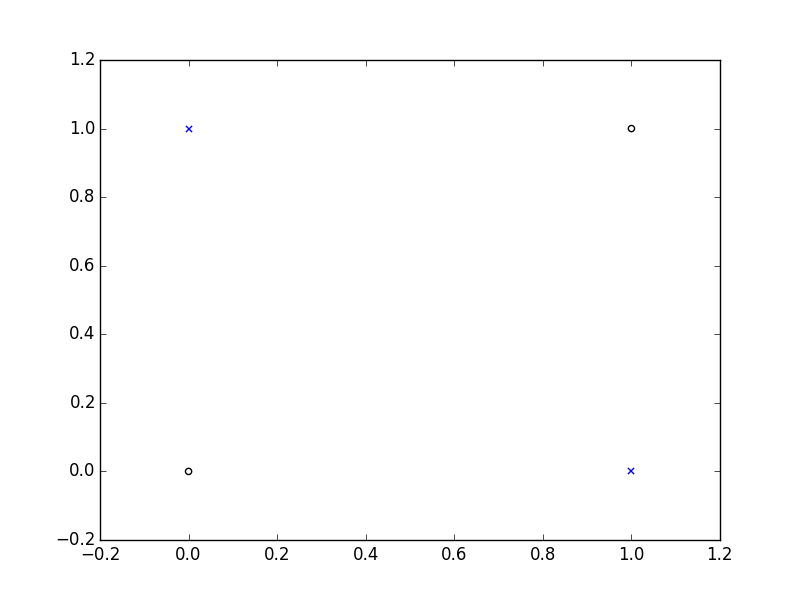
\includegraphics[width=\textwidth]{.//assets/images/xor.png}\caption{Figure Example}\label{fig:xor}\end{figure}

\section{Gist}\label{gist}

\inputminted[mathescape, linenos, frame=lines, framesep=2mm]{Python}{.gist-cache/cache.7aeefc0de1bb10005514355a5c4a5dfe-1c74b8336494cb0e9c6d-xor-5d.py}

\section{Post Link}\label{post-link}

\href{http://localhost:4000/2015/04/29/foo/}{Foo}

Awesome paper\cite{mikolov2013efficient}.

\bibliographystyle{unsrt}

\bibliography{assets/printables/references}

\renewcommand{\thefootnote}{}

\footnotetext{Online version at \url{http://localhost:4000/2015/04/29/foo/}}

\end{document}
